\RequirePackage{fix-cm}
\documentclass[twocolumn]{svjour3}          % twocolumn
\journalname{Behavior Research Methods}


%\documentclass[jou,apacite]{apa6}
%\shorttitle{Online behavioral research with psiTurk}
%
%\twoauthors{Author One}{Author Two}
%\twoaffiliations{Institute of Psychology}{Freud's Institute}
%
%\abstract{psiTurk is really great and you should use it.}
%
%\rightheader{Online behavioral research with psiTurk}
%\leftheader{Online behavioral research with psiTurk}

\usepackage{listings}
\usepackage{color}
\usepackage{graphicx}

\definecolor{dkgreen}{rgb}{0,0.6,0}
\definecolor{gray}{rgb}{0.5,0.5,0.5}
\definecolor{mauve}{rgb}{0.58,0,0.82}

\lstset{frame=tb,
  %language=Java,
  aboveskip=5mm,
  belowskip=5mm,
  showstringspaces=false,
  columns=flexible,
  basicstyle={\ttfamily},
  numbers=none,
  numberstyle=\tiny\color{gray},
  keywordstyle=\color{blue},
  commentstyle=\color{dkgreen},
  stringstyle=\color{mauve},
  frame=none,
  breaklines=true,
  breakatwhitespace=true
  tabsize=3
}

\begin{document}

\title{psiTurk: A framework for running behavioral experiments online}

\author{First Author         \and
        Second Author %etc.
}


%\authorrunning{Short form of author list} % if too long for running head

\institute{F. Author \at
              first address \\
              Tel.: +123-45-678910\\
              Fax: +123-45-678910\\
              \email{fauthor@example.com}           %  \\
%             \emph{Present address:} of F. Author  %  if needed
           \and
           S. Author \at
              second address
}

\date{Received: date / Accepted: date}

\maketitle

\begin{abstract}
Insert your abstract here.
\keywords{Online experiments \and open science}
\end{abstract}

\section{Introduction (AC)}

Online experiments are growing in popularity. 
They offer a number of advantages over lab-based experiments, as well as novel technical and experimental challenges.

psiTurk is a framework of software and web services that facilitate the creation, running, and dissemination of web-based experiments.
It presently relies on Amazon Mechanical Turk to recruit and pay participants on the web.
It solves a number of technical requirements including serving an experiment on the web, saving experimental data, and restricting the participant pool according to the experimenter's needs.
The principal goal of this framework is thus to handle common technical challenges so that researchers can focus on the development and dissemination of online experiments.

\section{Web-based behavioral research}

\subsection{Survey of researchers' needs (AR)}

In early 2014 we conducted a survey to assess the methods and needs of behavioral researchers with
respect to online experiments.  We collected responses from 201 researchers in psychology (58\%),
linguistics (16\%), marketing (7\%), neuroscience (6\%), and economics (4\%), most of whom had some
experience collecting behavioral data online in their labs (85\%).

These researchers showed a clear interest in online data collection. Nearly all listed fast data
collection (98\%) and large sample sizes (93\%) as benefits of online data collection, with most
interested in the potential for lower costs (75\%) and a more diverse population (60\%) as well. Nearly
40\% stated that they treat papers reporting data collected online identically to that collected in
a lab.

\begin{figure*}[tp]
\centering
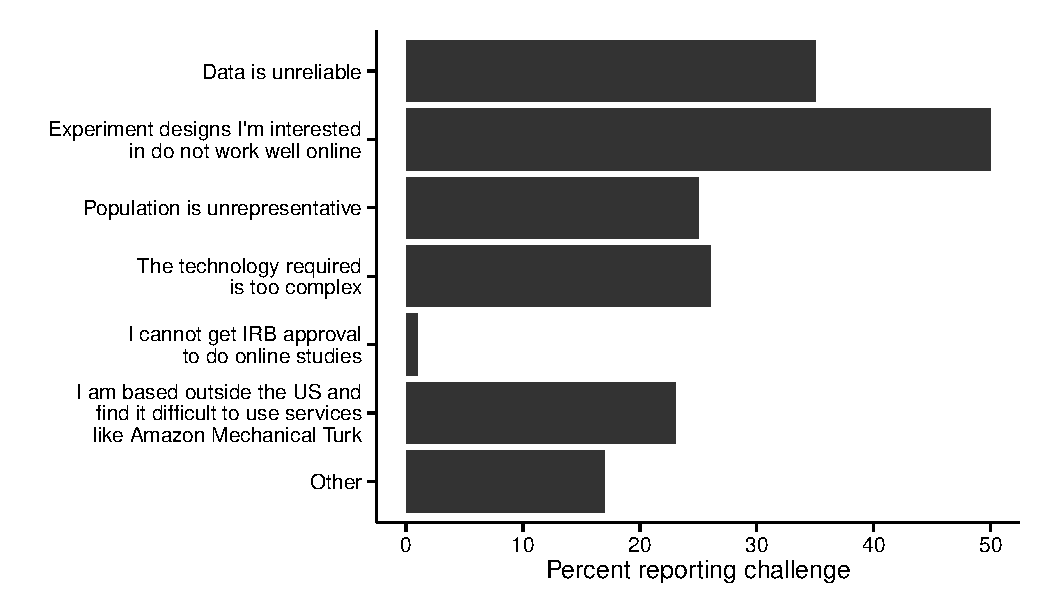
\includegraphics[scale=.75]{figures/challenges.pdf}
\caption{Challenges faced by 201 researchers who completed our survey on collecting behavioral data online.}
\label{fig:challenges}
\end{figure*}

Respondents also felt that online data collected presented a set of unique challenges, as shown in
Figure~\ref{fig:challenges}. Some felt that data collected online was unreliable (35\%) or the
population unrepresentative (25\%). Many felt that experiment designs they were interested in did
not work well online (50\%), or that web technology is too complex (25\%), and researchers based
outside the US reported difficulty using services like Amazon Mechanical Turk (23\%).


The majority of respondents (56\%) listed Qualtrics, a service for conducting online surveys, as the tool they
were currently most likely to use, but most (79\%) expressed interest in being able to run full
experiments including multiple, trials, fixation crosses, etc. The vast majority (94\%) reported
interest in new tools that simplified online data collection.


\subsection{Amazon Mechanical Turk (AMT)} 

Amazon Mechanical Turk (AMT) is an online platform that lets you post a wide variety of tasks to a large pool of participants.
Instead of spending weeks to run experiments in the lab, it lets you collect data of a large number of people within a couple of hours.
Workers get paid a fixed amount for each HIT which is determined by the requester.

\subsubsection{From the worker's perspective (JVM)}
AMT functions as an online listing service for online jobs.
Workers search through a list of tasks, known as Human Intelligence Tasks (HITs). 
When a worker examines a particular task, they are able to see metadata about the task, such as its title and how much it pays, and a website provided by the requester inside a web frame.
This website serves as an advertisement for the task and must be hosted either by Amazon or on the requester's hosted servers.
Once a worker has accepted a HIT, he or she agrees to complete it within a particular amount of time.
The actual task is again served either from Amazon or the requester's own hosted service.
The hosting both serves the job to the worker and collects data.
Finally, the worker is returned the AMT worker page to be credited and continue to another HIT.

\subsubsection{From the requester's perspective (TMG)}
Requesters can also make bonus payments to specific workers. Amazon collects a 10\% fee for each payment.
AMT provides some very basic templates that you can use to design HITs (particularly questionnaires), but these will most likely not serve your purposes as an experimenter.
The psiTurk toolbox is designed to help you run fully-customized and dynamic web-experiments on AMT.
Specifically, it allows you to:
1. Run a web server for your experiment
2. Test your experiment
3. Interact with AMT to recruit, post HITs, filter, and pay participants (AMT workers)
4. Manage databases and export data
psiTurk also includes a powerful interactive command interface that lets you manage most of your AMT activity.


\subsection{What problems does psiTurk solve? (AC)}

Brief overview of how psiTurk addresses needs/challenges raised in the previous sections, before going on to a more detailed walkthrough in the next section.


\subsubsection{Better/More efficient interface to AMT}

Automatic bonusing

Simplifies paying participants quickly, including bonuses


\subsubsection{Technical complexity and security}

No need for dedicated server

No need to install, configure and maintain complex webserver software (e.g., Apache, MySQL)

Flexible database options

Includes industry standards (Bootstrap, jQuery, d3, etc)

Custom routes

Minimize security issues since server only runs while you want to collect data

Secure Ad server

\subsubsection{Tailored to behavioral research}

Ability to filter browsers, iPhones, tablets, etc. 

Automatically fill in conditions randomly and evenly

Templates (consent, instructions, errors, debrief)

Prevent same worker from performing your experiment multiple times




\subsection{Remaining challenges}

Some of the concerns raised by survey respondents are inherent to online data collection.
Reliability of data. 
Note existing research about whether online experiments replicate lab versions.

Do certain experiments not work well online?
Requires careful consideration depending on the specific experimental design.

Return to these challenges at the end of the paper.


%\begin{table*}[t]
%\caption{default}
%\begin{center}
%\begin{tabular}{|l|l|l|}
%Category & Issue & psiTurk solution \\
%\hline
%Participant pool & Preventing repeated participation in same experiment & Database \\
%\end{tabular}
%\end{center}
%\label{default}
%\end{table*}%



\section{Overview of the psiTurk system}

The structure of the psiTurk system is shown in Figure X.

AMT

psiTurk experiment server (local computer)

Ad server

Experiment exchange

\subsection{Configuration and project structure}

AMT keys.

psiTurk keys.

Anatomy of a psiturk experiment folder.


\subsection{Command line interface: Managing HITs and serving the experiment (AR)}

PsiTurk runs as a command line interface (CLI) within a standard terminal window.
There are several advantages to designing psiTurk as a simple CLI beyond its efficiency of use. This
design makes the user-interface code clear and easy to read and write, allowing newcomers to quickly
understand and contribute to the open-source project. Integrating a new feature into the interface
is as simple as describing the syntax and functioning of a new command. The CLI also ensures that
psiTurk is easy to interact with not just on a laptop or desktop but also on a remote server or in
the cloud, where users may have terminal-only access.
 
Entering
\texttt{psiturk} at the command line in any directory containing a psiTurk project launches the
psiTurk CLI.
The psiTurk CLI features a colorized prompt that provides important information at a glance, including
whether the server is running, the current mode (``live" or ``sandbox", and the number of HITs currently running on AMT:

\begin{lstlisting}
[psiTurk server:off mode:sdbx #HITs:0]$
\end{lstlisting}

\noindent In some examples below, this prompt is truncated as \texttt{[psiTurk]\$} to indicate commands that occur within the psiTurk CLI, while commands that are entered on the command line are preceded simply by \texttt{\$}.


\subsubsection{Managing HITs}
Commands are organized into groups based on their function, following a general ``\texttt{command subcommand
arguments}'' format. For example, one can create a HIT by typing 

\begin{lstlisting}
[psiTurk]$ hit create <# assignments> <$ amount> <duration>
\end{lstlisting}

What happens after you create a HIT?

%\noindent or list all active HITs with 
%
%\begin{lstlisting}
%[psiTurk]$ hit list --active
%\end{lstlisting}

Can restart the server with \texttt{server restart} or open the server log with \texttt{server log}. 
Tab completion makes it quick to type commands, and the \texttt{help} command can be used to show
details on the usage of any command. 
The straightforward and consistent syntax of the CLI allows
users to perform a wide variety of tasks--from creating HITs and paying workers, to launching Amazon
Web Services database instances, to opening an experiment in a browser for debugging--that
would otherwise be spread across a number of websites and programs. 
Easily switch between AMT's sandbox and live site.

In most cases, a user of the
psiTurk CLI will never have to log into the MTurk website except to add money to their MTurk
requester account.



\subsubsection{Serving an experiment}

The experiment server is started using

\begin{lstlisting}
[psiTurk]$ server on
\end{lstlisting}


psiTurk experiments can be hosted on almost anything that has an internet connection and a public port, such as an office computer or laptop.
You'll need a static IP to prevent your experiment's URL from changing. 
Users without one (e.g., most home users) can use a dynamic DNS service to forward a URL to their dynamic IP.
Here's a list of free DDNS providers.
You also may need to forward a port from your home routers to you personal computer.
To run your experiment in a web browser you need to have at least some basic web programming skills (especially using HTML, CSS, and JavaScript).
Once you mastered the basics, you can take advantage of the vast number of libraries and tools that can help you to build sharp and sophisticated experiments with the support of a large community of users.
To get you started, psiTurk provides a fully functioning example experiment (Getting up and running with the basic Stroop task) that you can use as a template for your own study.


\subsection{The Ad server}

PsiTurk helps an experimenter in both hosting the ad and delivering the experiment.
First, PsiTurk provides a cloud service at \texttt{psiturk.org} for serving ads to workers.
This service serves the ads with appropriate SSL certificates, something which can be difficult on many server configurations.\footnote{SSL certification has recently become a requirement for hosting content within an \texttt{iframe} on \texttt{mturk.com}.}
Second, the PsiTurk web framework allows you to easily build and host your own experiment, running on your server or laptop and saving workers' data either to your own database  or to \texttt{psiturk.org}.
This gives experimenters complete flexbility in terms of content while also offering a suite of tools to make experiment development easy.

SSL hosted Ad Server removes need to deal with complex web security issues (https, data mining on workers) 
Participants recruited via Mechanical Turk first interact with your task via ads. Ads are simply the digital version of hanging a poster or flyer around your university building in order to recruit participants. Technically, ads are snippets of HTML code that describe what your task is about and what you're offering for compensation. As a result, they are the front line for any subject recruitment online. It's easy to overlook the importance of a good ad, and making that ad visible to as many participants as possible.




%Extendable Python based API: easily add new functionality
%
%Library of experiments you can adapt or replicate
%
%Fully open-source development helps catch bugs
%
%Since everything runs locally easy to debug/test (even w/o Internet!)
%
%Run experiments on local computer (via tunnel) (can run offline and online)
%
%Perfect for laboratory-based courses with undergrads (replicating studies)



\subsection{Javascript library \emph{psiTurk.js} (DBM)}

The javascript library \emph{psiTurk.js} enables interaction with the server from the client-side (javascript) experiment code.
The goal of the library is to handle the most common functionality of psiTurk-based web experiments, without imposing any additional requirements on the structure or design of the experiments themselves.
Researchers can draw on a vast array of javascript libraries to design their experiment, while using psiTurk.js to save data and notify the server of changes in a participant's status.

Figure X shows javascript code from an experiment script (\emph{task.js}). 
\emph{psiTurk.js} currently performs the following functions:


\subsubsection{Tracking a participant's progress in an experiment} 

psiTurk records changes in a participant's status as they move through an experiment. 
Some of these status changes are automatic, e.g., when a participant is assigned to a condition or if they quit an experiment early. 
Two additional status changes are initiated by the client-side experiment code using psiTurk.js functions.
First, since experiments typically begin with an instructional phase, calling the function \texttt{psiturk.finishInstructions()} upon completion of this phase will save the participant's status as having begun the main experiment.
If the participant attempts to quit the experiment after that point, they will receive a warning that they will not be able to restart the experiment and may forgo payment.
Second, successful completion of the experiment is signaled by calling \texttt{psiturk.completeHIT()}, which closes the experiment and redirects the participant to the AMT page to submit their HIT.

\subsubsection{Saving experimental data} 

Experiment code can save data in two formats.
\texttt{psiturk.recordTrialData} takes any array of values as input and appends it to a list of ``trial" data.
This data structure is meant for sequential data that may be collected over the course of multiple trials or blocks, where each line corresponds to a new measurement.
However, the format of this data is defined by the experimenter and is saved in the database as a single JSON object.

In contrast, \texttt{psiturk.recordUnstructuredData} is used to record (key, value) pairs, where the key is uniquely defined within the experiment.
This format is useful for survey questions or other one-time measurements, e.g., (\emph{Age}: 24).

Importantly, both functions above simply record the data in the appropriate format on the client-side.
When the experimenter wishes to save the data to the server they call \texttt{psiturk.saveData}.

\subsubsection{Automatic recording of browser interaction}
 
One general shortcoming of web experiments is greater uncertainty about a participant's testing environment and engagement with the experiment.
Unlike lab computers where undesired behaviors can be prevented, a person is always able to close a web browser, switch to different applications, or change other aspects of their experience.
However, standard methods exist for recording many aspects of a user's interaction with a web browser, and this data can be useful for 1) tracking how an experiment was actually displayed, and 2) the level of a participant's engagement.

For example, although it is possible to set the initial size of a browser window, a web participant can change the dimensions of the window, potentially obscuring or altering how the experiment is displayed.
\emph{psiTurk.js} automatically records these changes in the size of the window.
Similarly, the experiment can choose to switch focus away from the experiment window (e.g., to another browser window or a different application).
\emph{psiTurk.js} automatically records every time that the experiment window loses and gains the participant's focus.
This ``event data" is automatically recorded and saved to the database whenever \texttt{psiturk.saveData} is invoked. \\


\emph{psiTurk.js} can also preload html pages and images.
Finally, it has a basic structure for presenting instructional pages.

\subsection{Experiment exchange}

A significant advantage of web-based experiments is the potential for low-friction replication and extension. 
The \emph{experiment exchange} (EE, found at http://psiturk.org/ee) facilitates the sharing of experiments that have been built to run using psiTurk, acting as an ``app store" for psiTurk-compatible designs.
Once an experiment has been completed, a researcher can submit the following information to register their experiment on the exchange:

\begin{enumerate}
\item A Github repository containing the experiment code
\item Metadata about the experiment, including a title, description, and keywords
\item The DOI for any paper describing the results of the experiment (if any)
\item The version of psiTurk that was used to run the experiment
\end{enumerate}


Metadata associated with an experiment allows other researchers to discover it through the psiTurk website.
A publicly available experiment can then be downloaded using the following command on the command line,

\begin{lstlisting}
$ psiturk-install <experiment-specific-id>
\end{lstlisting}

\noindent with the experiment-specific identifier found on the exchange page.
If psiTurk is already configured on the user's system, the downloaded experiment will run without further changes, and can then act as a starting point for direct replication or extensions.
Modified versions can then be re-run using the same population via AMT, thereby minimizing the potential for experimenter-specific biases.

Other initiatives (e.g., the Open Science Framework, https://osf.io) also aim to improve the transparency, reproducibility, and efficiency of research through centralized services, but are less focused on the specific technology involved in running online experiments.
In contrast, the psiTurk experiment exchange links together experiments that can be run within a common framework.
As a result, existing experiments can serve as examples to help new researchers learn to code for the web; they shorten the development time necessary (especially for popular experimental paradigms); and the exchange facilitates communication between researchers with similar interests.

\section{Limitations and future directions (TMG)}

Some challenges that were noted by the survey are inherent to online data collection 

Restriction to AMT, can be an unrepresentative participant pool. 

No Windows

Counterbalancing (integrate PlanOut (Facebook's counterbalancing tool)) (DH)

Optimal Experimental Design/ Design of Experiments tools

Better multi-person/multi-session exp (websockets; doug?)?

Automate catch trials? How far did the worker get? Do we count them in the N? 

Limiting/throttling number of people doing the experiment at once

Video support

%\bibliography{sample}

\end{document}
